\textbf{Цели работы:} изучение поляризации света при отражении и преломлении; нахождение степени поляризации лазерного излучения.

\textbf{Приборы и принадлежности:} экспериментальная установка для изучения поляризации света, представляющая собой модульный учебный комплекс по волновой оптике (МУК-ОВ).

Установка состоит из механического и электронного блоков (рис. 4.8). Механический блок 1 представляет собой основание 10, на котором установлены и закреплены: стойка 17, служащая вертикальной оптической скамьей; турель 19; защитный экран 18; электронный блок 5. На стойке смонтированы оптические узлы 2--4, 16, которые могут вращаться и выводиться из поля зрения, если при выполнении эксперимента они не используются. Защитный экран 18 не вращается и участвует во всех экспериментах на данной установке.

Электронный блок 5 содержит кнопки, индикаторы измерительных устройств и окна фотоприемников.

При выполнении данной лабораторной работы используются следующие узлы механического блока 1: защитный экран 18, поляризатор 2, устройство для измерения угла Брюстера 4 с матовой полупрозрачной шкалой, анализатор 16. Вращающаяся втулка на устройстве 4 позволяет изменять угол падения луча на стеклянную пластинку относительно вертикальной шкалы. Поляризатор 2 и анализатор 16 снабжены угломерной шкалой. На электронном блоке 5 используются: кнопка включения лазера 12; регулятор интенсивности 13; кнопка переключения фотоприемников 8; индикатор относительной интенсивности света 7; четыре индикатора включенного фотоприемника 14 с определенным диапазоном длин волн; кнопка включения электронного блока «Сеть» 9 и окно фотоприемника лазерного излучения 6.

\begin{figure}[H]
    \def\thefigure{4.8}
    \protect\phantomsection 
	
    \centering
    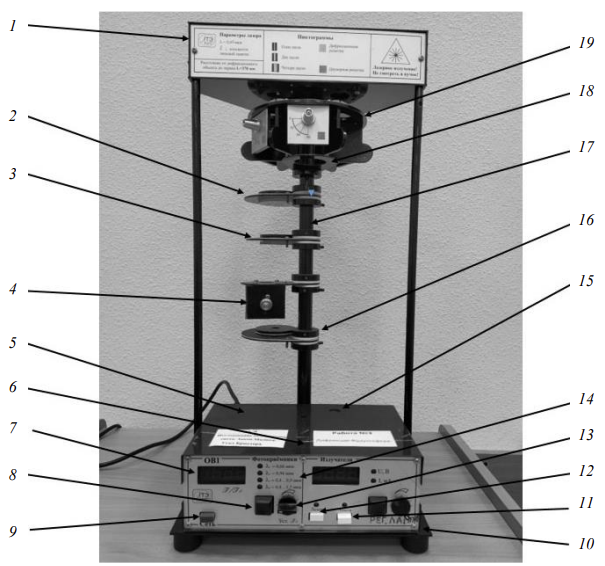
\includegraphics[width=0.8\linewidth]{figs/1.png}
	\caption{Экспериментальная установка по волновой оптике (МУК-ОВ)}
	\label{fig:exp_setup}
\end{figure}

В лабораторной установке на индикаторе 7 показывается не абсолютная, а относительная интенсивность излучения $I_{\varphi} = I/I_0$, где $I_0$ -- некоторая константа, задаваемая чувствительностью измерительного прибора.

\newpage
\centeredsection{\MakeUppercase{Исследуемые закономерности}}
В данной работе проводится проверка закона Малюса, определяется степень поляризации лазерного излучения и находится показатель преломления стекла через угол Брюстера.

\subsection*{1. Проверка закона Малюса и определение степени поляризации}

\subsubsection*{Теоретическая основа:}
Интенсивность $I$ плоскополяризованного света, прошедшего через анализатор, зависит от угла $\varphi$ между плоскостью поляризации света и плоскостью пропускания анализатора согласно закону Малюса:

\begin{equation}
    I(\varphi) = I_{max} \cdot \cos^2{\varphi}
    \label{eq:malus_law}
\end{equation}
где $I_{max}$ --- максимальная интенсивность света, прошедшего через анализатор.

Степень поляризации $P$ для частично поляризованного света определяется по формуле:

\begin{equation}
    P = \frac{I_{max} - I_{min}}{I_{max} + I_{min}}
    \label{eq:degree_of_polarization}
\end{equation}
где $I_{min}$ --- минимальная интенсивность.

\subsubsection*{Порядок действий и обработка:}
\begin{enumerate}
    \item \textbf{Снятие данных для закона Малюса:} Пропустив луч лазера через поляризатор и анализатор, измерьте зависимость относительной интенсивности $I_\varphi$ от угла поворота анализатора $\varphi$ с шагом в 10$^\circ$.
    
    \item \textbf{Обработка:} Постройте на миллиметровой бумаге экспериментальный график зависимости нормированной интенсивности $I_\varphi(\varphi)/I_{\varphi, max}$ от угла $\varphi$. Сравните его с теоретической зависимостью $y = \cos^2{\varphi}$, построенной на том же графике.
    
    \item \textbf{Определение степени поляризации:} Найдите максимальное ($I_{\varphi, max}$) и минимальное ($I_{\varphi, min}$) значения интенсивности, вращая анализатор. Рассчитайте степень поляризации $P$ по приведённой выше формуле.
\end{enumerate}

\subsection*{2. Определение угла Брюстера и показателя преломления}

\subsubsection*{Теоретическая основа:}
При падении света на границу раздела двух диэлектриков под \textbf{углом Брюстера} $\theta_Б$ отраженный луч становится полностью плоскополяризованным, а его интенсивность --- минимальной. Угол Брюстера связан с показателем преломления $n$ вещества \textbf{законом Брюстера}:

\begin{equation}
    \tan(\theta_\text{Б}) = n
    \label{eq:bruster_law}
\end{equation}

\subsubsection*{Порядок действий и обработка:}
\begin{enumerate}
    \item \textbf{Измерение:} На пути лазерного луча установите стеклянную пластину на поворотном устройстве. Изменяя угол падения луча $\theta$, визуально найдите такое его значение, при котором интенсивность отраженного луча будет минимальной.
    
    \item \textbf{Обработка:} Измеренный угол падения, при котором наблюдается минимум интенсивности, является углом Брюстера $\theta_\text{Б}$. Вычислите показатель преломления $n$ материала пластины по формуле $n = \tan(\theta_\text{Б})$.
\end{enumerate}



















\newpage
\centeredsection{\MakeUppercase{Указания по проведению эксперимента}}

\textbf{1. Нахождение степени поляризации излучения лазера.}
\begin{enumerate}
    \item[1.1.] Включить лазерный источник света, соблюдая правила техники безопасности (не допускать прямого попадания лазерного излучения в глаз). Турель 19 (рис. 4.8) установить так, чтобы излучение от источника проходило ее беспрепятственно.
    \item[1.2.] Кнопкой переключения фотоприемников 8 установить диапазон длин волн $\lambda_4 = 0.4...1.2$ мкм, о чем будет свидетельствовать включение одного из индикаторов 14. Вращением ручки 13 добиться наибольших показаний максимальной относительной интенсивности $I_{\varphi} = I/I_0$ на индикаторе 7 (рис. 4.8).
    \item[1.3.] Поскольку выходящий из лазерного источника свет является эллиптически-поляризованным, то для превращения его в плоскополяризованный на пути лазерного луча поместить поляризатор 2. Стрелку шкалы поляризатора установить на $0^\circ$.
    \item[1.4.] Установить между лазером и фотоприемником анализатор 16.
    \item[1.5.] Вращая анализатор и непрерывно следя за показаниями цифрового индикатора интенсивности, измерить максимальное ($I_{\varphi\ max}$) и минимальное ($I_{\varphi\ min}$) значения относительной интенсивности проходящего излучения. Наблюдения выполнить 5 раз и результаты записать в протокол.
\end{enumerate}

\textbf{2. Проверка закона Малюса.}
\begin{enumerate}
    \item[2.1.] Схема установки (рис. 4.8) для проверки закона Малюса состоит из источника света -- лазера, поляризатора 2, анализатора 16, фотоприемника 6. Правила включения лазерного источника и настройки установки не меняются и соответствуют пп. 1.1--1.4.
    \item[2.2.] Вращая анализатор, снять зависимость относительной интенсивности $I_\varphi(\varphi)$ от угла поворота анализатора $\varphi$ через каждые $10^\circ$ от $\varphi = -150^\circ$ до $\varphi = +150^\circ$, проходя через $0^\circ$ (вращать против часовой стрелки). Результаты наблюдений занести в протокол.
\end{enumerate}

\textbf{3. Нахождение угла Брюстера для стеклянной пластинки.}
\begin{enumerate}
    \item[3.1.] Схема установки (см. рис. 4.8) по определению угла Брюстера для стеклянной пластинки состоит из источника света -- лазера, поляризатора 2, устройства для измерения угла Брюстера 4 с матовой полупрозрачной вертикальной шкалой и фотоприемника 6. В данном эксперименте анализатор 16 не используется, поэтому его нужно установить в положение вне хода лазерного луча. Правила включения лазерного источника и настройки установки не меняются и соответствуют пп. 1.1--1.3.
    \item[3.2.] Установить по ходу луча устройство для измерения угла Брюстера 4.
    \item[3.3.] Вращая втулку на устройстве 4, визуально пронаблюдать за изменениями интенсивности луча лазера, отраженного от стеклянной пластинки под углом $\theta$, фиксируемым на вертикальной шкале.
    \item[3.4.] Добиться минимальной интенсивности луча, визуально наблюдаемого при отражении от стеклянной пластинки, что соответствует падению светового луча на стеклянную пластинку под углом Брюстера. Определить по шкале числовое значение полученного угла $\theta_Б$. Результат наблюдений занести в протокол.
    \item[3.5.] Выключить установку кнопкой «Сеть» 9.
\end{enumerate}




















\newpage
\thispagestyle{empty}
\centeredsection{ПРОТОКОЛ НАБЛЮДЕНИЙ}

\begin{table}[H]
    \centering
    \caption{Измерение максимальной и минимальной интенсивности ($\theta_I=0.01$)}
    \label{tab:polarization}
    \begin{tabular}{|c|c|c|}
        \hline
            № & $\qquad I_{max} \qquad$ & $\qquad I_{min} \qquad$   \\
        \hline
            1 & 0.051 & 0.000 \\
        \hline
            2 & 0.076 & 0.000 \\
        \hline
            3 & 0.052 & 0.000 \\
        \hline
            4 & 0.075 & 0.000 \\
        \hline
            5 & 0.053 & 0.000 \\
        \hline
    \end{tabular}
\end{table}

\begin{table}[H]
    \centering
    \caption{Зависимость интенсивности от угла анализатора}
    \label{tab:protocol:malus_law_corrected}
    \begin{tabularx}{\linewidth}{|c|c|C||c|c|C|}
        \hline
        \textbf{$\varphi$, $^{\circ}$} & \textbf{$\cos^2\varphi$} & \textbf{$I_\varphi \cdot 10^3$} & \textbf{$\varphi$, $^{\circ}$} & \textbf{$\cos^2\varphi$} & \textbf{$I_\varphi \cdot 10^3$} \\
        \hline
        0 & 1.000 & 50 & 80 & 0.030 & 2 \\
        \hline
        10 & 0.970 & 48 & 90 & 0.000 & 0 \\
        \hline
        20 & 0.883 & 48 & 100 & 0.030 & 2 \\
        \hline
        30 & 0.750 & 38 & 110 & 0.117 & 8 \\
        \hline
        40 & 0.587 & 33 & 120 & 0.250 & 19 \\
        \hline
        50 & 0.413 & 23 & 130 & 0.413 & 29 \\
        \hline
        60 & 0.250 & 14 & 140 & 0.587 & 43 \\
        \hline
        70 & 0.117 & 8 & 150 & 0.750 & 55 \\
        \hline
    \end{tabularx}
\end{table}

\begin{table}[H]
    \centering
    \caption{Измерение угла}
    \label{tab:angle}
    \begin{tabular}{|c|c|}
        \hline
            № & $\qquad \Theta_i, {}^\circ \qquad$\\
        \hline
            1 & 65\\
        \hline
            2 & 64 \\
        \hline
            3 & 63 \\
        \hline
    \end{tabular}
\end{table}

\vfill
\noindent
Рахметов А. Р., гр. 4494 ~~\hrulefill~~ «\rule{1cm}{0.4pt}» \rule{3cm}{0.4pt} 20\rule{0.75cm}{0.4pt} г.










\newpage
\centeredsection{Обработка результатов}

\subsection*{ \boxed{\text{ Задание 1.}} }
\begin{quote}
    \textit{Исходя из результатов наблюдений найти степень поляризации $P_i$ согласно \cref{eq:degree_of_polarization} для каждого наблюдения. Рассчитать результат измерения $P = \bar{P} \pm \Delta \bar{P}$.}
\end{quote}

Используя данные из \cref{tab:polarization}, рассчитаем степень поляризации для каждого из пяти измерений. Поскольку во всех случаях измеренное значение минимальной интенсивности $I_{min} = 0$, для каждого измерения получаем:
$$
P_i = \frac{I_{max, i} - 0}{I_{max, i} + 0} = 1
$$

Среднее значение степени поляризации составляет:
$$
\bar{P} = \frac{1}{5}\sum_{i=1}^{5} P_i = 1
$$

Случайная погрешность, определяемая разбросом данных, равна нулю, так как все $P_i = 1$. Расчитаем итоговую погрешность:
$$
\Delta P = \sqrt{ \left( \frac{\partial P}{\partial I_{max}} \Delta I_{max} \right)^2 + \left( \frac{\partial P}{\partial I_{min}} \Delta I_{min} \right)^2 }
$$
где $\Delta I_{max} = \Delta I_{min} = \theta_I = 0.01$. Частные производные равны:
$$
\frac{\partial P}{\partial I_{max}} = \frac{2 I_{min}}{(I_{max} + I_{min})^2}; \qquad \frac{\partial P}{\partial I_{min}} = \frac{-2 I_{max}}{(I_{max} + I_{min})^2}
$$

Для расчета необходимо среднее значение максимальной интенсивности:
$$
\bar{I}_{max} = \frac{0.051 + 0.076 + 0.052 + 0.075 + 0.053}{5} = \frac{0.307}{5} = 0.0614
$$

Подставим $\bar{I}_{max} = 0.0614$ и $\bar{I}_{min} = 0$ в выражения для производных:
$$
\frac{\partial P}{\partial I_{max}} = \frac{2 \cdot 0}{(0.0614 + 0)^2} = 0
$$
$$
\frac{\partial P}{\partial I_{min}} = \frac{-2 \cdot 0.0614}{(0.0614 + 0)^2} = -\frac{2}{0.0614} \approx -32.57
$$

Теперь можно рассчитать погрешность $\Delta P$:
$$
\Delta P = \sqrt{ (0 \cdot 0.01)^2 + (-32.57 \cdot 0.01)^2 } = 32.57 \cdot 0.01 = 0.3257
$$

В результате получаем:
$$
P = 1.0 \pm 0.3257
$$
$$
P = 1.0 \pm 0.3
$$

\begin{flushright}
    \boxed{\text{Ответ: }P = 1.0 \pm 0.3}
\end{flushright}



\subsection*{ \boxed{\text{ Задание 2. }} }
\begin{quote}
    \textit{По результатам наблюдений (\cref{tab:protocol:malus_law_corrected}) найти максимальное значение $I_{\varphi, max}$, рассчитать значения отношения $I_\varphi / I_{\varphi, max}$ для каждого значения угла $\varphi$ и построить на миллиметровой бумаге график зависимости $I_\varphi/I_{\varphi, max}$ от угла $\varphi$. Сравнить полученный экспериментальный график с теоретическим графиком, построенным согласно заданиям по подготовке к работе (п. 3).}
\end{quote}

Согласно закону Малюса: $I(\varphi) = I_{\varphi, max} \cdot \cos^2{\varphi} \Longrightarrow \frac{I(\varphi)}{I_{\varphi, max}} = \cos^2{\varphi}$.
Из \cref{tab:protocol:malus_law_corrected} видно, что $I_{\varphi, max} = 50 \cdot 10^{-3}$ при $\varphi = 0^\circ$.
Рассчитаем $I_\varphi/I_{\varphi, max}$ для всех значений угла $\varphi$:

\begin{table}[H]
    \centering
    \caption{Сравнение экспериментальных данных с законом Малюса}
    \label{tab:malus_law_processed}
    \begin{tabularx}{\linewidth}{|c|c|C||c|c|C|}
        \hline
            $\varphi$, $^{\circ}$ &
            $\cos^2\varphi$ (теор.) &
            $I_\varphi/I_{\varphi, max}$ (эксп.) &
            $\varphi$, $^{\circ}$ &
            $\cos^2\varphi$ (теор.) &
            $I_\varphi/I_{\varphi, max}$ (эксп.) \\
        \hline
            0  & 1.000 & 1.000 & 80  & 0.030 & 0.040 \\
        \hline
            10 & 0.970 & 0.960 & 90  & 0.000 & 0.000 \\
        \hline
            20 & 0.883 & 0.960 & 100 & 0.030 & 0.040 \\
        \hline
            30 & 0.750 & 0.760 & 110 & 0.117 & 0.160 \\
        \hline
            40 & 0.587 & 0.660 & 120 & 0.250 & 0.380 \\
        \hline
            50 & 0.413 & 0.460 & 130 & 0.413 & 0.580 \\
        \hline
            60 & 0.250 & 0.280 & 140 & 0.587 & 0.860 \\
        \hline
            70 & 0.117 & 0.160 & 150 & 0.750 & 1.100 \\
        \hline
    \end{tabularx}
\end{table}


\subsection*{ \boxed{\text{ Задание 3. }} }
\begin{quote}
    \textit{Используя полученное экспериментально значение угла Брюстера (\cref{tab:angle}) и формулу $\tan(\theta_\text{Б}) = n$, вычислить значение показателя преломления стеклянной пластинки устройства 4 (см. \cref{fig:exp_setup})}.
\end{quote}

Для вычисления показателя преломления сначала найдем среднее значение угла Брюстера по данным из \cref{tab:angle}:
$$
\bar{\theta}_Б = \frac{65^\circ + 64^\circ + 63^\circ}{3} = \frac{192^\circ}{3} = 64^\circ
$$
Теперь, используя закон Брюстера, вычислим значение показателя преломления стеклянной пластины:
$$
n = \tan(\bar{\theta}_Б) = \tan(64.0^\circ) \approx 2.0503
$$
Округляя результат до разумного числа значащих цифр (соответствующего точности исходных данных), получаем:
\begin{flushright}
    \boxed{n \approx 2.05}
\end{flushright}



\subsection*{Выводы}
Полученная погрешность в задании 1 является значительной. Вероятнее всего, что это связано с величиной приборной погрешности ($\theta_I=0.01$) по сравнению с измеряемыми значениями интенсивности ($\bar{I}_{max} = 0.0614$).

Как видно из \cref{tab:malus_law_processed}, экспериментальные значения в целом согласуются с теоретической зависимостью $\cos^2\varphi$, особенно вблизи $\varphi=0^\circ$ и $\varphi=90^\circ$. Наблюдаемые расхождения, особенно при больших углах, могут быть вызваны погрешностями установки нуля на угловой шкале анализатора и неточностями при снятии показаний. Тем не менее, общая тенденция подтверждает справедливость закона Малюса.

Полученное значение показателя преломления $n \approx 2.05$ является аномально высоким для обычного стекла ($n \approx 1.5 \div 1.7$). Такое расхождение указывает на наличие существенной погрешности в эксперименте.




















% \newpage
% \centeredsection{Вопросы}
% \section*{Вопрос 1.}
% \begin{quote}
%     \textit{Поляризатор, анализатор, полероид --- ?}
% \end{quote}

% \begin{enumerate}
%     \item Поляризатор --- это оптическое устройство, предназначенное для получения поляризованного (упорядоченного) света из естественного (хаотичного).
%     \item Анализатор --- устройство, которое позволяет определять, поляризован свет или нет, и регулировать его интенсивность.
%     \item Поляроид (поляризационный светофильтр) --- это тип линейного поляризатора, представляющий собой тонкую дихроичную плёнку, заключенную между двумя прозрачными пластинами.
%         \begin{itemize}
%             \item Линейный поляризатор --- это оптическое устройство, предназначенное для преобразования неполяризованного (естественного) света в плоскополяризованный свет (т.е. $\vec{E}$ колеблется строго в одной плоскости, перпендикулярной направлению распространения волны).
%             \item Дихроизм --- это физическое явление, при котором оптический материал поглощает две линейно-поляризованные, взаимно перпендикулярные составляющие падающего на него света по-разному, что позволяет устранять блики, регулировать яркость, анализировать поляризационное состояние света.
%         \end{itemize}
% \end{enumerate}





% \section*{Вопрос 2.}
% \begin{quote}
%     \textit{Вращение плоскости полеризации}
% \end{quote}

% Вращение плоскости поляризации --- это физическое явление, заключающееся в повороте вектора поляризации плоскополяризованного света вокруг направления его распространения при прохождении через определённые среды.

% Явление вращения плоскости поляризации (оптическая активность) объясняется теорией Френеля.
% Линейно поляризованный свет ($\vec{E}$) можно представить как суперпозицию двух круговых поляризованных волн --- правополяризованной ($R$) и левополяризованной ($L$).
% В оптически активных средах (например, в растворе сахара) существует разница в показателях преломления для этих двух компонент ($\Delta n = n_L - n_R \neq 0$).
% Из-за этой разницы волны $R$ и $L$ распространяются с разными скоростями и приобретают разность фаз ($\Delta \varphi$) при прохождении пути $l$.
% При их повторном сложении на выходе плоскость результирующей линейно поляризованной волны оказывается повернутой на угол $\alpha$, который описывается формулой: 
% $$\alpha = \frac{\pi l}{\lambda} (n_L - n_R),$$
% где $\lambda$ — длина волны света.
% Для растворов этот угол также пропорционален концентрации $C$ вещества и длине пути $l$ по закону Био: $\alpha = [\alpha] \cdot l \cdot C$, где $[\alpha]$ — удельное вращение.


\newpage
\centeredsection{Вопросы}
\section*{Вопрос 1.}
\begin{quote}
    \textit{Поляризатор, анализатор, поляроид --- ?}
\end{quote}

\begin{enumerate}
    \item \textbf{Поляризатор и анализатор} — это физически идентичные устройства, различающиеся лишь своей функцией и положением в оптической схеме.
        \begin{itemize}
            \item \textbf{Поляризатор} — оптический элемент, который преобразует естественный (неполяризованный) свет в линейно-поляризованный. Его основное свойство — наличие \textit{оси пропускания}. Он пропускает только ту составляющую вектора напряженности электрического поля $\vec{E}$, которая параллельна этой оси, а перпендикулярную составляющую поглощает или отражает. Поляризатор всегда стоит первым на пути естественного света.
            
            \item \textbf{Анализатор} — тот же поляризатор, но используемый для \textit{анализа} состояния поляризации света, прошедшего через поляризатор и, возможно, исследуемую среду. Вращая анализатор, можно определить плоскость поляризации и степень поляризации света, наблюдая за изменением интенсивности по закону Малюса.
        \end{itemize}
    
    \item \textbf{Поляроид} (или поляризационный светофильтр) — это наиболее распространенный на практике тип линейного поляризатора. Его работа основана на явлении \textit{дихроизма}.
        \begin{itemize}
            \item \textbf{Дихроизм} — это свойство некоторых кристаллов по-разному поглощать свет в зависимости от его поляризации.
            \item Поляроид представляет собой тонкую полимерную пленку с внедренными в нее микроскопическими дихроичными кристаллами, которые ориентированы параллельно друг другу. Такая структура эффективно поглощает свет, поляризованный в одном направлении, и почти без потерь пропускает свет с перпендикулярной поляризацией.
        \end{itemize}
        Другие типы поляризаторов, в отличие от поляроидов, могут работать на иных принципах, например, на двойном лучепреломлении (призма Николя) или на отражении света под углом Брюстера.
\end{enumerate}

\section*{Вопрос 2.}
\begin{quote}
    \textit{Вращение плоскости поляризации}
\end{quote}

Вращение плоскости поляризации (или оптическая активность) — это физическое явление, заключающееся в повороте плоскости поляризации линейно-поляризованного света при его прохождении через определенные вещества, называемые оптически активными.

\begin{enumerate}
    \item Причиной оптической активности является \textit{хиральность} — структурная асимметрия молекул вещества или его кристаллической решетки. Хиральные объекты несовместимы со своим зеркальным отражением, подобно левой и правой руке. Из-за этой асимметрии среда по-разному взаимодействует с право- и левоциркулярно поляризованным светом.
    
    \item Явление объясняется представлением линейно-поляризованной волны как суперпозиции (суммы) двух когерентных волн с круговой поляризацией, вращающихся в противоположных направлениях — правой ($R$) и левой ($L$). (Теория Френеля).
        \begin{itemize}
            \item В оптически неактивной среде показатели преломления для обеих волн одинаковы ($n_L = n_R$), и они распространяются с одной скоростью.
            \item В оптически активной (хиральной) среде показатели преломления для них различны ($n_L \neq n_R$). Это явление называется круговым двойным лучепреломлением.
        \end{itemize}
        
    \item В результате, из-за разности скоростей распространения, при прохождении пути $l$ в среде между левой и правой компонентами накапливается разность фаз. При их последующем сложении на выходе из среды плоскость колебаний результирующего линейно-поляризованного вектора оказывается повернутой на угол $\alpha$.
\end{enumerate}

Угол поворота $\alpha$ описывается формулой:
$$
\alpha = \frac{\pi l}{\lambda_0} (n_L - n_R)
$$
где $l$ — длина пути в среде, $\lambda_0$ — длина волны света в вакууме. В зависимости от знака разности $(n_L - n_R)$, вещества делят на:
\begin{itemize}
    \item \textit{правовращающие} ($n_L > n_R$, $\alpha > 0$ по часовой стрелке для наблюдателя),
    \item \textit{левовращающие} ($n_L < n_R$, $\alpha < 0$ против часовой стрелки).
\end{itemize}


\centeredsection{Задача №32.}
\begin{quote}
    \textit{Плоскопараллельная пластинка в $1/4$ волны вырезана из кварца и имеет толщину $d = 16$ мкм. На неё падает монохроматический свет с $\lambda = 589$ нм. Определить показатель преломления $n_e$ необыкновенного луча, если показатель преломления обыкновенного луча $n_o = 1.5442$.}
\end{quote}

\begin{enumerate}
    \item По условию, пластинка является четвертьволновой ($\lambda/4$). Это означает, что она создает оптическую разность хода, равную нечетному числу четвертей длины волны:
          $$
          \left.
          \begin{array}{l}
              \Delta = |n_e - n_0| \cdot d \\
              \Delta = (2m + 1) \frac{\lambda}{4}, \quad m\in\mathbb{N}_0
          \end{array}
          \right|
          \!\!\!\Rightarrow (2m + 1) \frac{\lambda}{4} = |n_e - n_0| \cdot d
          $$

    \item Кварц является положительным одноосным кристаллом $\Rightarrow n_e > n_0$ \Longrightarrow |n_e - n_0| = n_e - n_0$.
          $$ (2m + 1) \frac{\lambda}{4} = (n_e - n_0) \cdot d \Longrightarrow n_e = n_0 + \frac{(2m + 1)\lambda}{4d} $$

    \item Для определения порядка $m$ (целое число $0, 1, 2, \dots$) оценим величину $\frac{\lambda}{4d}$:
          $$ \frac{\lambda}{4d} = \frac{589 \cdot 10^{-9} \text{ м}}{4 \cdot 16 \cdot 10^{-6} \text{ м}} = \frac{589}{64 \cdot 10^3} \approx 0.009203 $$
    
    \item Разность $n_e - n_0$ для кварца (согласно справочникам) на этой длине волны составляет $0.009$. $n_e - n_0 = (2m + 1) \cdot 0.009203 \Longrightarrow (2m + 1) \approx 1 \Longrightarrow m = 0 \Rightarrow$ пластинка первого порядка.
    
    \item Используем формулу для $m=0$:
          $$ n_e = n_0 + \frac{\lambda}{4d}\qquad \Longrightarrow \qquad n_e = 1.5442 + 0.009203$$
          $$ n_e \approx 1.553403 $$
\end{enumerate}


\begin{flushright}
    \boxed{\text{Ответ: }$n_e \approx 1.5534$.}
\end{flushright}
